%Para compilar:
%dvips slide.dvi
%ps2pdf slide.ps

\documentclass{beamer}
\usepackage[utf8]{inputenc}
\usepackage[spanish]{babel}
\usepackage{graphicx}

%%%%%%%%%%%%%%%%%%%%%%%%%%%%%%%%%%%%%%%%%%%%%%%%%%%%%%%%%%%%%%%%%%%%%%%%%%%%%%%%%%%%%%%%%%%%

\newtheorem{definicion}{Definición}
\newtheorem{ejemplo}{Ejemplo}

%%%%%%%%%%%%%%%%%%%%%%%%%%%%%%%%%%%%%%%%%%%%%%%%%%%%%%%%%%%%%%%%%%%%%%%%%%%%%%%%%%%%%%%%%%%%

\usetheme{classic}
\usecolortheme[RGB={125,60,125}]{structure}

%%%%%%%%%%%%%%%%%%%%%%%%%%%%%%%%%%%%%%%%%%%%%%%%%%%%%%%%%%%%%%%%%%%%%%%%%%%%%%%%%%%%%%%%%%%%

\title[Integración]{Método del trapecio.}
\author[Grupo-2D]{Miriam Martín Jacinto.\\Tiffany López Nicholson.\\Sergio Vega García.}
\date[01/05/2013]{1 de mayo de 2013.}

%%%%%%%%%%%%%%%%%%%%%%%%%%%%%%%%%%%%%%%%%%%%%%%%%%%%%%%%%%%%%%%%%%%%%%%%%%%%%%%%%%%%%%%%%%%%

\begin{document}
%%%%%%%%%%%%%%%%%%%%%%%%%%%%%%%%%%%%%%%%%%%%%%%%%%%%%%%%%%%%%%%%%%%%%%%%%%%%%%%%%%%%%%%%%%%%
  \begin{frame}
    
\includegraphics[width=0.15\textwidth]{ull.eps}
    \hspace{7cm}
    
\includegraphics[width=0.15\textwidth]{fmatesc.eps}
    \titlepage
  \end{frame}
%%%%%%%%%%%%%%%%%%%%%%%%%%%%%%%%%%%%%%%%%%%%%%%%%%%%%%%%%%%%%%%%%%%%%%%%%%%%%%%%%%%%%%%%%%%%
  \begin{frame}
    \frametitle{Índice.}
    \tableofcontents[pausesections]
  \end{frame}
%%%%%%%%%%%%%%%%%%%%%%%%%%%%%%%%%%%%%%%%%%%%%%%%%%%%%%%%%%%%%%%%%%%%%%%%%%%%%%%%%%%%%%%%%%%%
  \section{Integración.}
  \begin{frame}
    \frametitle{Integración.}
      \begin{definicion}
	Una \textbf{integral} es una generalización de la suma de infinitos sumandos, infinitamente pequeños.
      \end{definicion}
	
      \begin{definicion}
	Dada una función f(x) y un intervalo [a,b], la \textbf{integral definida} es igual al área limitada entre la gráfica de f(x), el eje de abscisas, y las rectas verticales x = a y x = b.\\
	$\int_{a}^{b} f(x) dx$, continua en el intervalo $[a, b].$
      \end{definicion}
  \end{frame}
%%%%%%%%%%%%%%%%%%%%%%%%%%%%%%%%%%%%%%%%%%%%%%%%%%%%%%%%%%%%%%%%%%%%%%%%%%%%%%%%%%%%%%%%%%%%
  \section{Regla del trapecio.}
  \begin{frame}
    \frametitle{Regla del trapecio.}
    \begin{definicion}
      La \textbf{regla del trapecio} es un método de integración numérica que se basa en aproximar el valor de la integral definida de $f(x)$ por el de la función lineal que pasa a través de ésta, formándose una figura: un trapecio. Para obtener esta aproximación, debemos calcular el área de los trapecios.
    \end{definicion}
  \end{frame}
%%%%%%%%%%%%%%%%%%%%%%%%%%%%%%%%%%%%%%%%%%%%%%%%%%%%%%%%%%%%%%%%%%%%%%%%%%%%%%%%%%%%%%%%%%%%
  \section{Nuestro caso.}
  \begin{frame}
    \begin{block}{La integral.}
      En esta exposición se mostrará la siguiente integral utilizando la \textbf{regla del trapecio} y nuestro programa $Python$.\\
      \begin{center}
	$\int_{1}^{6}\frac{1}{1+e^x}dx$, en el intervalo $[1,6]$
      \end{center}
    \end{block}

    \begin{block}{¿Qué vamos a hacer?}
      Crearemos un algoritmo en \textbf{$Python$} para hacer varias pruebas utilizando la regla del trapecio, obteniendo distintos resultados dependiendo de las partciones que haremos.
    \end{block}
  \end{frame}
%%%%%%%%%%%%%%%%%%%%%%%%%%%%%%%%%%%%%%%%%%%%%%%%%%%%%%%%%%%%%%%%%%%%%%%%%%%%%%%%%%%%%%%%%%%%
  \section{Algoritmo.}
  \begin{frame}
    \frametitle{Algoritmo.}
    \begin{block}{Comienzo.}
      Para empezar, se tendrá que observar que hace la función $f(x)=\frac{1}{1+e^{x}}$ en el intervalo $[1, 6]$.
      Ahora, se deberá estudiar la función utilizando la \textbf{regla del trapecio}.
      \begin{center}
	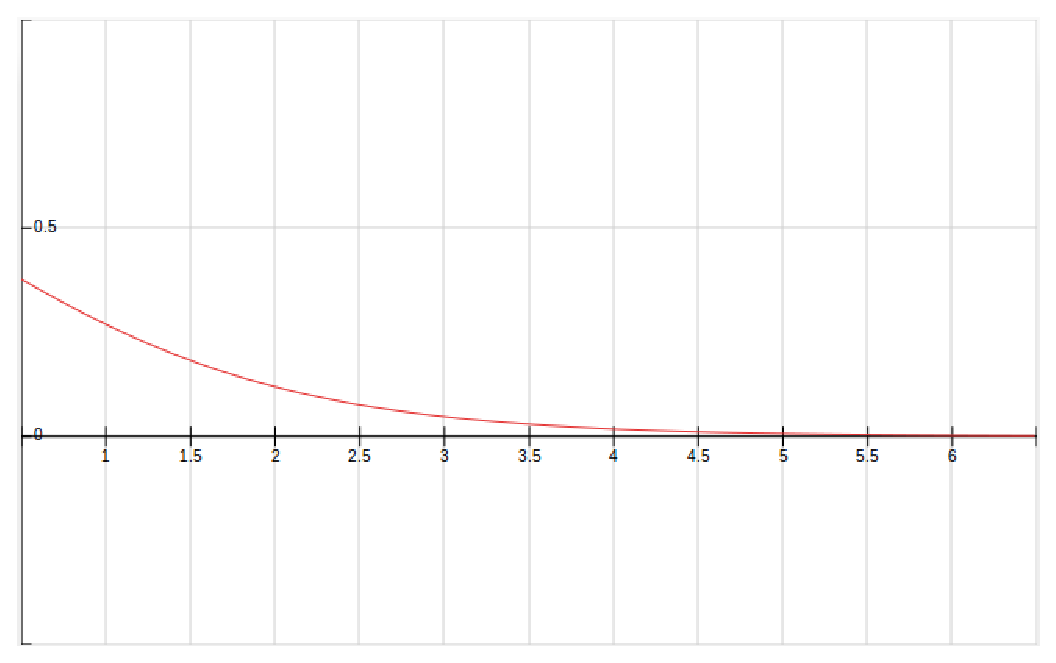
\includegraphics[width=0.5\textwidth]{img4.eps}
      \end{center}
    \end{block}
  \end{frame}
%%%%%%%%%%%%%%%%%%%%%%%%%%%%%%%%%%%%%%%%%%%%%%%%%%%%%%%%%%%%%%%%%%%%%%%%%%%%%%%%%%%%%%%%%%%%
  \begin{frame}
    \begin{block}{ }
      \begin{itemize}
	\item Se creará un programa en $Python$ capaz de implementar el teorema, eligiendo el número de particiones que el usuario introduce.
	\pause
	\item Aun así, más tarde se querrá hacer más comparaciones; por tanto, se añade al programa la opción de elegir un intervalo de particiones.
	\pause
	\item Además, se quiere comprobar el tiempo que tarda en implementar el algoritmo en una computadora.
      \end{itemize}
    \end{block}
  \end{frame}
%%%%%%%%%%%%%%%%%%%%%%%%%%%%%%%%%%%%%%%%%%%%%%%%%%%%%%%%%%%%%%%%%%%%%%%%%%%%%%%%%%%%%%%%%%%%
  \begin{frame}
    \begin{center}
      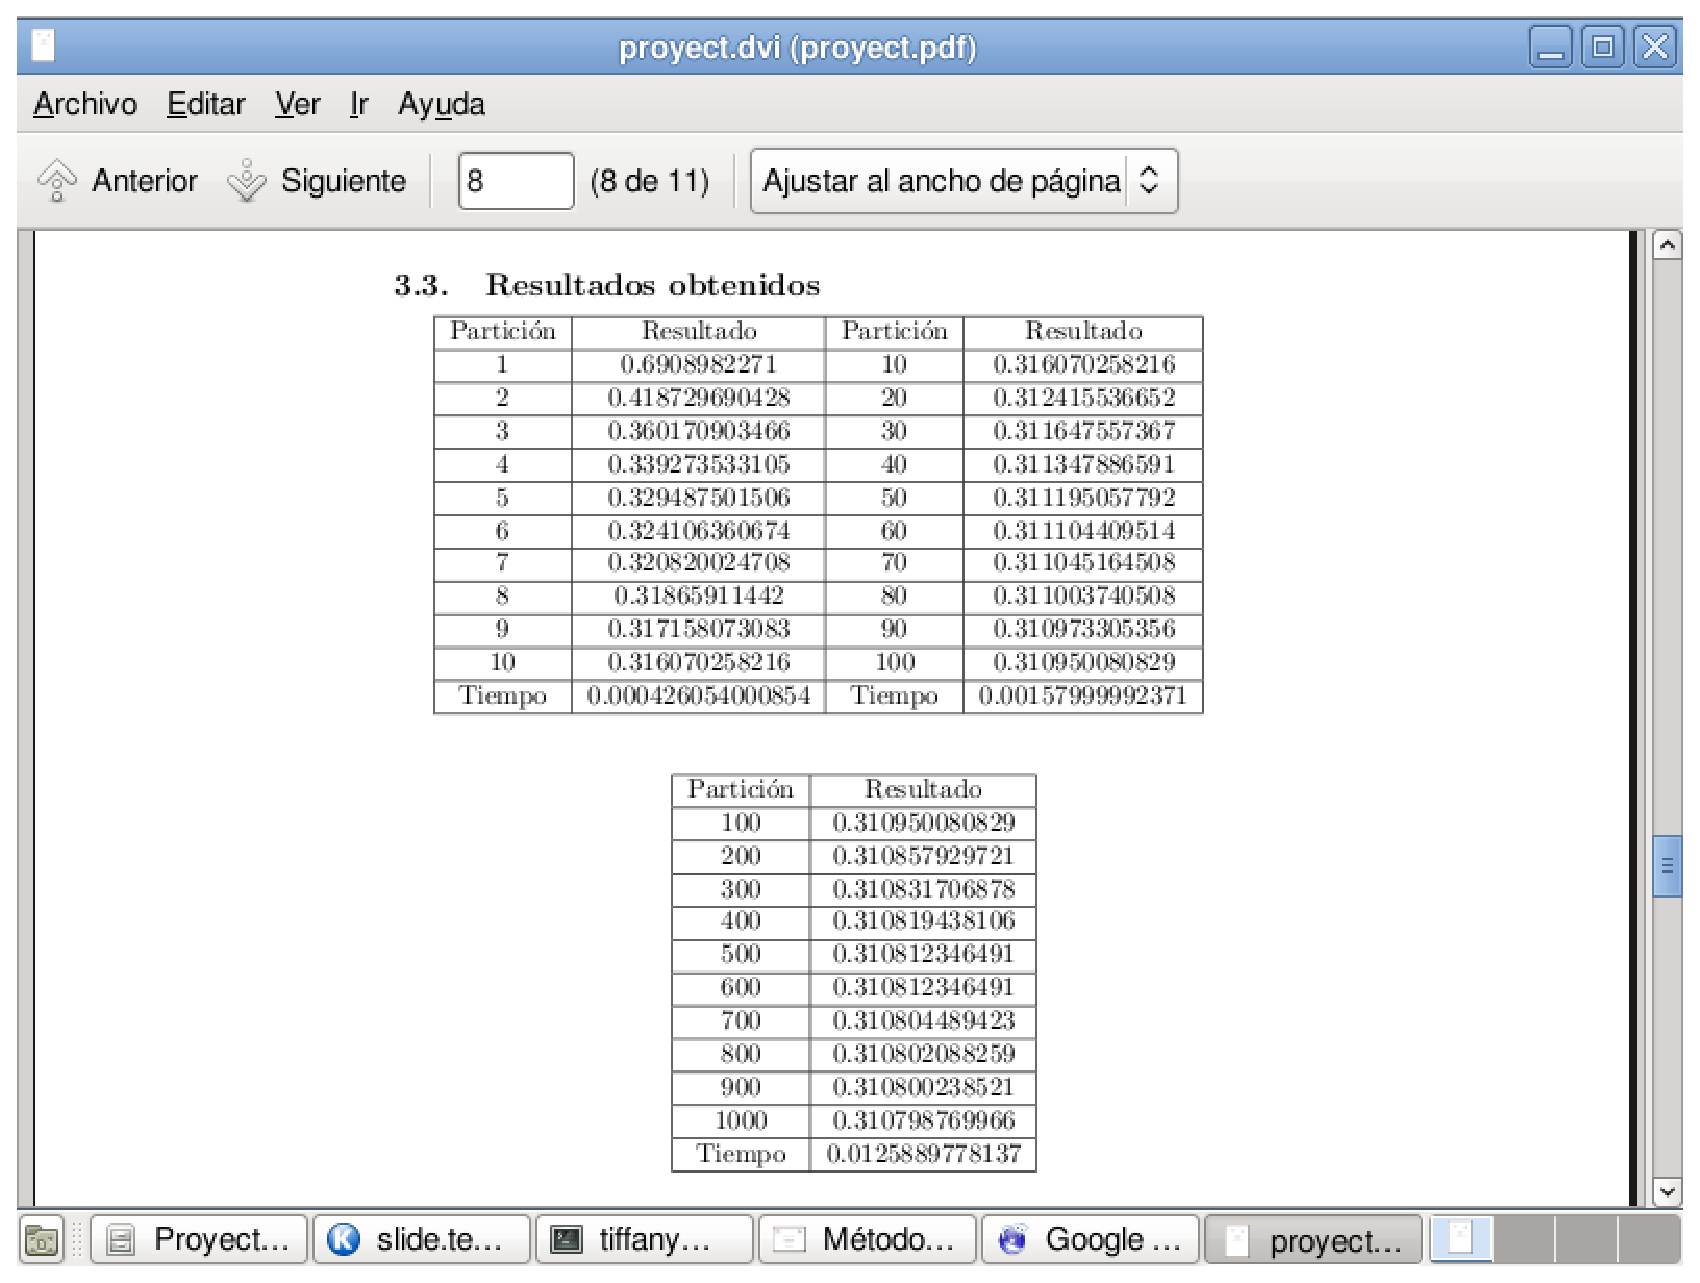
\includegraphics[width=0.9\textwidth]{img1.eps}
    \end{center}
  \end{frame}
%%%%%%%%%%%%%%%%%%%%%%%%%%%%%%%%%%%%%%%%%%%%%%%%%%%%%%%%%%%%%%%%%%%%%%%%%%%%%%%%%%%%%%%%%%%%
  \section{Conclusiones.}
  \begin{frame}
    \frametitle{Conclusiones.}
    \begin{enumerate}
      \item 
      La función determina la cantidad mínima de particiones para una buena aproximación de la función. \pause
      \item
      Muy útil para funciones complicadas, sobre todo si utilizamos un programa informático como $Python$. \pause
      \item
      Para funciones más sencillas, será mejor utilizar la tabla de \textit{integrales inmediatas} para hallar la solución.
    \end{enumerate}
  \end{frame}
%%%%%%%%%%%%%%%%%%%%%%%%%%%%%%%%%%%%%%%%%%%%%%%%%%%%%%%%%%%%%%%%%%%%%%%%%%%%%%%%%%%%%%%%%%%%
  \section{Bibliografía.}
  \begin{thebibliography}{00}
    \bibitem{trap}
      Regla del trapecio. $http://es.wikipedia.org/wiki/Regla\_del\_trapecio$
    \bibitem{int}
      Integración:\\ \emph{http://math2.org/math/integrals/es-tableof.htm}
    \bibitem{}
      Símbolos en \LaTeX:\\ \emph{http://web.ift.uib.no/Teori/KURS/WRK/TeX/symALL.html}
    \bibitem{Lag}
      Interpolación polinómica de Lagrange:\\ \emph{http://es.wikipedia.org/wiki/Interpolacion\_polinomica\_de\_Lagrange}
    \bibitem{Wei}
      Teorema de aproximación de Weierstrass:\\ \emph{http://es.wikipedia.org/wiki/Teorema\_de\_aproximacion\_de\_Weierstrass}
    \bibitem{num}
      Integración numérica:\\ \emph{http://portales.puj.edu.co/objetosdeaprendizaje/Online/OA10/capitulo4/capitulo4\_2.htm}
  \end{thebibliography}

%%%%%%%%%%%%%%%%%%%%%%%%%%%%%%%%%%%%%%%%%%%%%%%%%%%%%%%%%%%%%%%%%%%%%%%%%%%%%%%%%%%%%%%%%%%%

\end{document}

%%%%%%%%%%%%%%%%%%%%%%%%%%%%%%%%%%%%%%%%%%%%%%%%%%%%%%%%%%%%%%%%%%%%%%%%%%%%%%%%%%%%%%%%%%%%
